\linespread{0.4}
\documentclass[10pt,a5paper]{extarticle}
\usepackage[utf8]{inputenc}
\usepackage[T2A]{fontenc}
\usepackage[bulgarian]{babel}
\usepackage{grbbridge}
\usepackage{amsmath}
\usepackage{multicol}
\usepackage{xcolor}
\usepackage{mathptmx}
\usepackage{mdframed}
\usepackage{tikz}
\usepackage{tabularx}\usepackage[normalem]{ulem}
\usepackage[margin=1in]{geometry}
\usepackage[normalem]{ulem} % better underlines

%------------------- New commands ---------------------%

\newcommand{\Rheart}{\textcolor{red}{\heartsuit}}
\newcommand{\Rdiamond}{\textcolor{orange}{\diamondsuit}}
\newcommand{\Bspade}{\textcolor{black}{\spadesuit}}
\definecolor{darkgreen}{RGB}{0,70,0}
\newcommand{\Bclub}{\textcolor{darkgreen}{\clubsuit}}
\newcommand{\NT}{\text{NT}}
\newcommand{\leadhil}[1]{\textcolor{red}{\uline{#1}}}

%------------------- Header - Footer -------------------%
\usepackage{fancyhdr}

\pagestyle{fancy}
\fancyhf{} % clear all header/footer fields
\fancyhead[R]{
    
\includegraphics[width=4mm, height=4mm]{images/su_logo_imagelarge.jpg}
Факултет по математика и информатика} % right header
\setlength{\headheight}{8pt} % height of header
\setlength{\headsep}{10pt}    % space between header and text
\fancyfoot[C]{\thepage}


%---------------------------------------------------------------------------%

\begin{document}

\begin{titlepage}
    \centering
    
\includegraphics[width=0.3\textwidth]{images/su_logo_imagelarge.jpg} % optional logo
    \vfill
    {\Huge\bfseries Натурална система за начинаещи \par}
    \vfill
    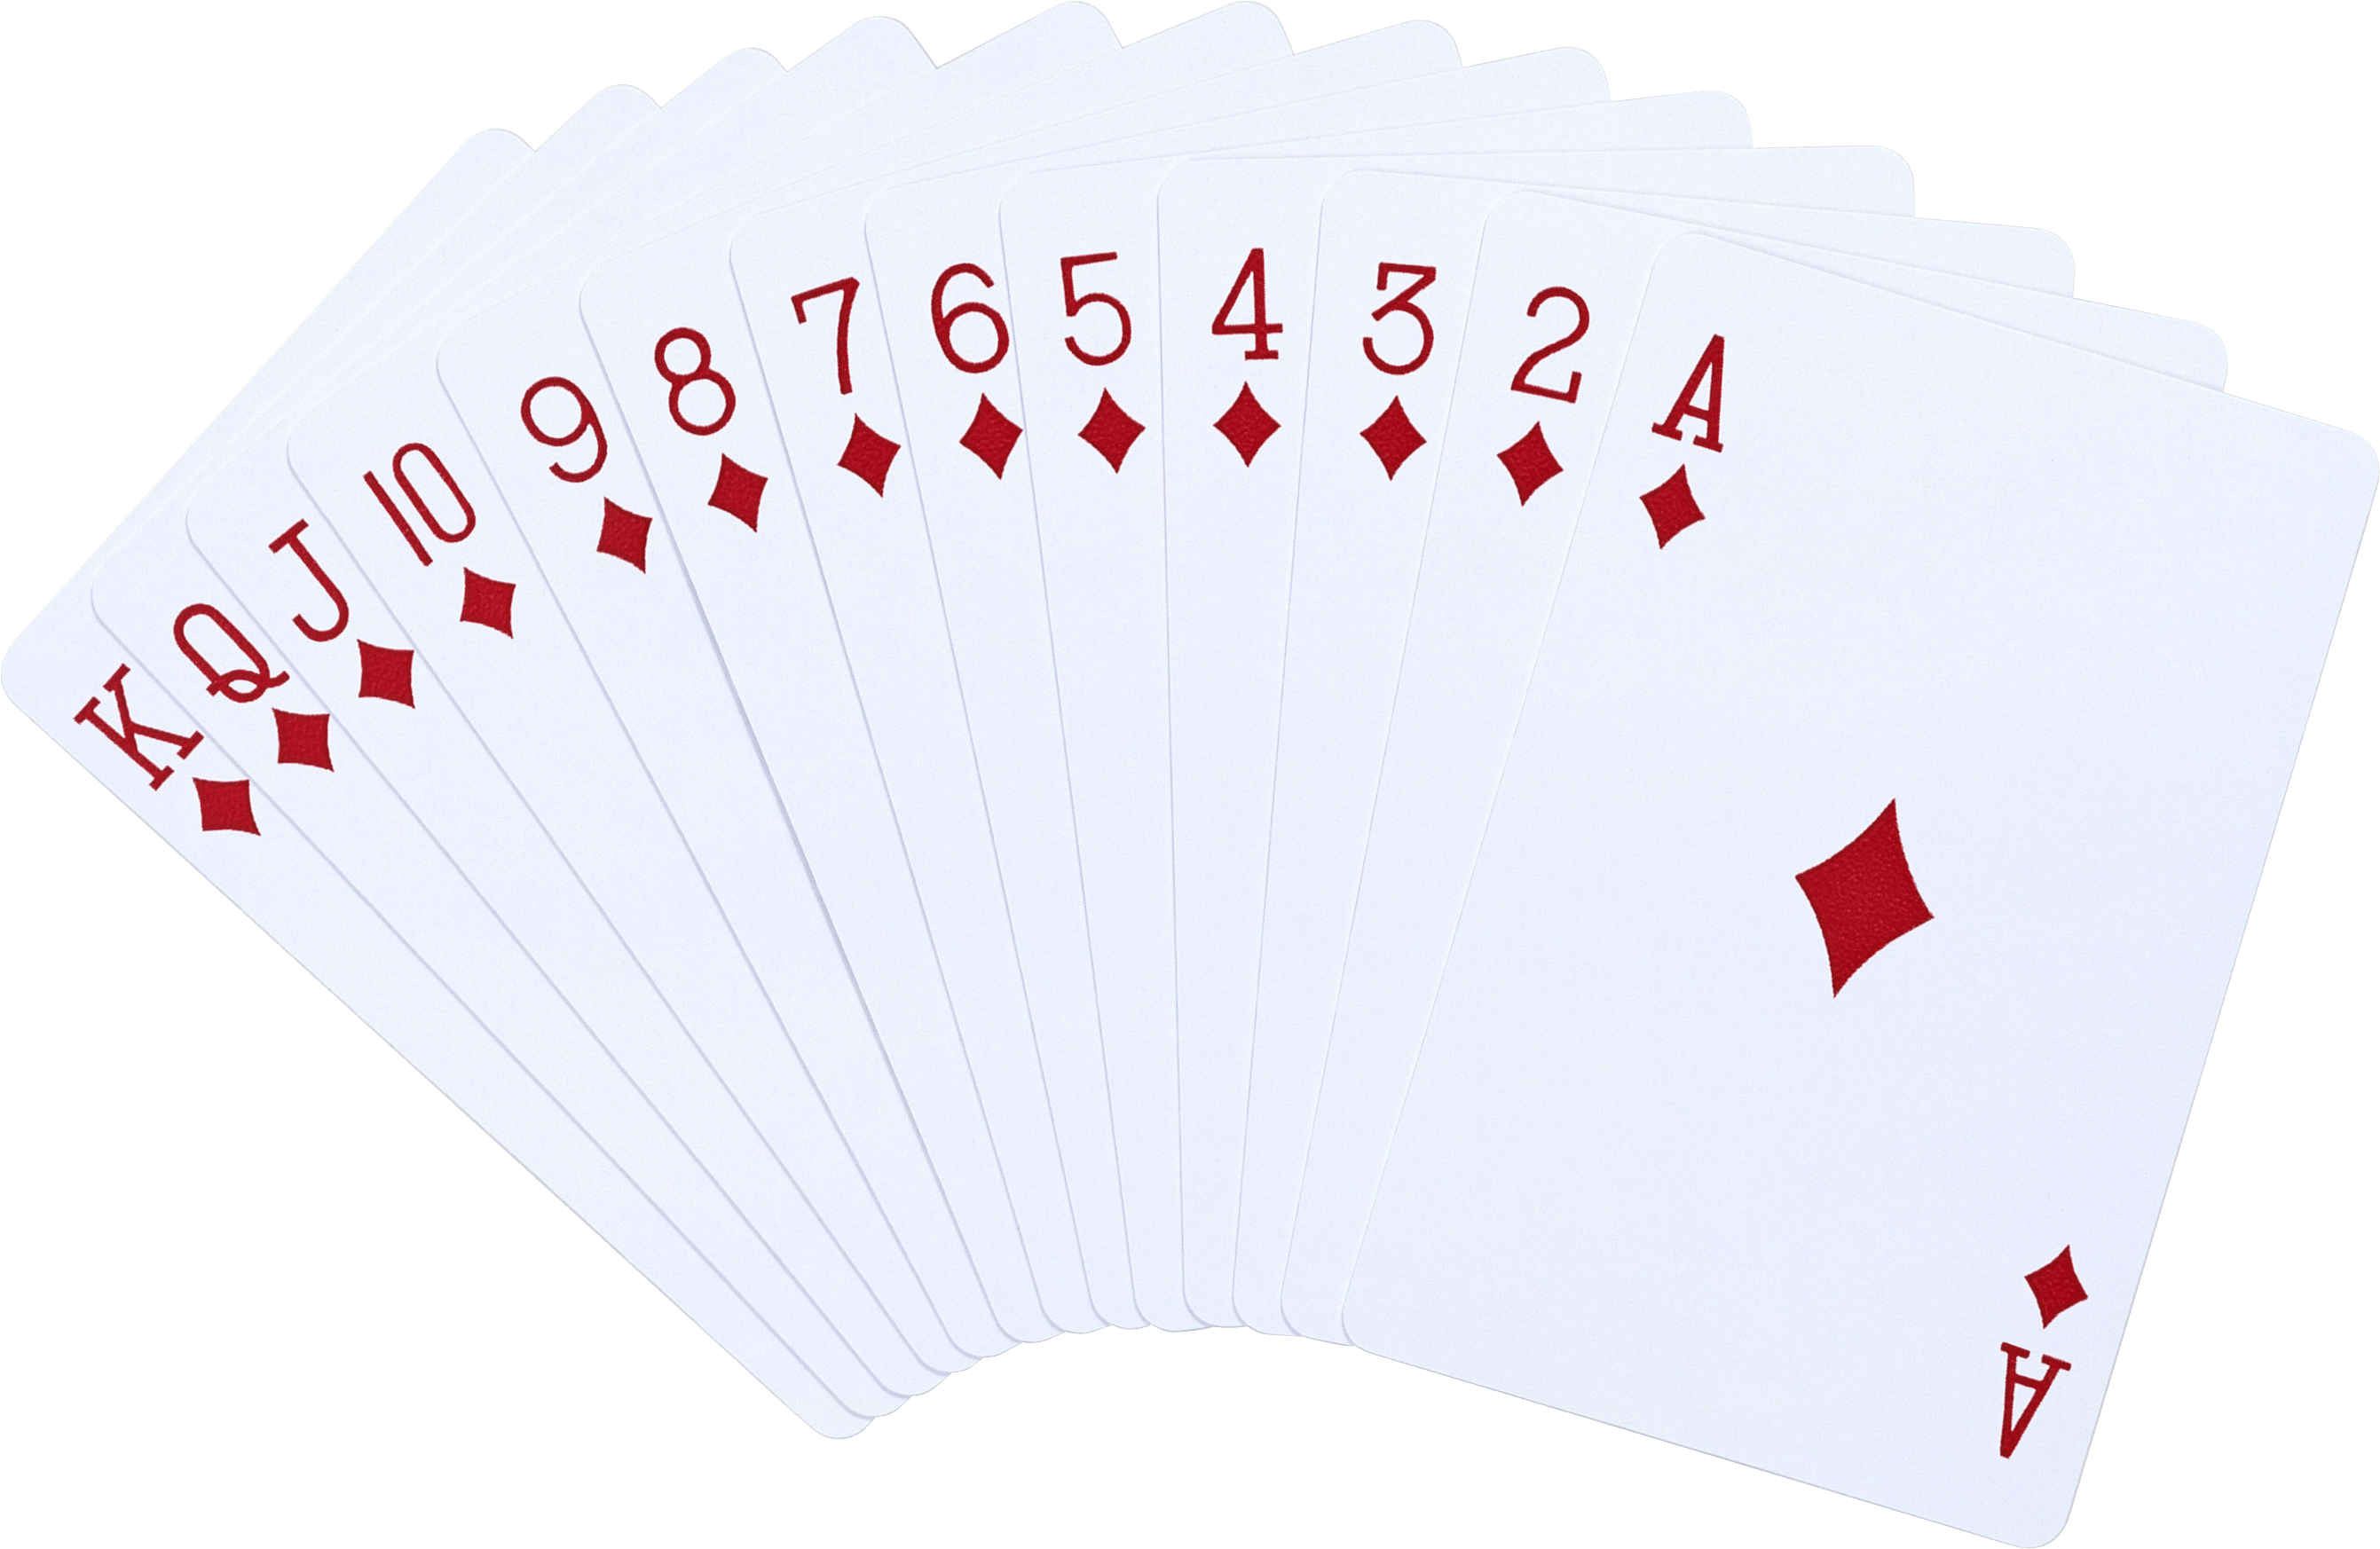
\includegraphics[width=0.8\textwidth]{images/diamonds.png} % optional logo
    \vfill
    {\large bridgecup.vercel.app \par}
\end{titlepage}

\newpage

\tableofcontents

\section*{Общи принципи}
\addcontentsline{toc}{section}{Общи принципи} % Add to TOC

\begin{itemize}
    \item[] Всички откривания на 1-во ниво са натурални.
    \item[] Откриванията 1$\Rheart$ и 1$\Bspade$ показват 5+ карти в цвета.
    \item[] Откриваме с най-дългия цвят:
        \begin{itemize}
            \item[] при 5-4 с петорния,
            \item[] при 6-5 с шесторния цвят.
        \end{itemize}
    \item[] С два 5-картови или два 6-картови цвята откриваме с по-високия по ранг: $\Bspade\ > \Rheart\ > \Rdiamond\ > \Bclub$.
    \item[] При липса на 5-картов мажор:
        \begin{itemize}
            \item[] с 4-4 в минорите откриваме 1$\Rdiamond$,
            \item[] с 3-3 в минорите откриваме 1$\Bclub$.
        \end{itemize}
    \item[] Откриване 2$\Bclub$ е условен силен анонс (единственото форсиращо откриване в системата).
    \item[] Откриванията 1БК, 2БК и 3БК показват балансирани ръце (4333, 4432 и 5332).
    \item[] Всички по-високи откривания на ниво 2/3/4/5 са натурални баражи.
    \item[] Стилът на преговорите (по-нататъшното анонсиране от двамата партньори) е натурален.
    \item[] Повечето първи отговори след откриване 1 в цвят са натурални.
    \item[] В системата се ползват малък брой общоприети и разпространени конвенции:
        \begin{itemize}
            \item[] Stayman,
            \item[] Transfers след безкозови откривания,
            \item[] Jacoby 2БК след откриване 1 в Мажор,
            \item[] Takeout double и Negative doubles,
            \item[] Blackwood.
        \end{itemize}
\end{itemize}

\vspace{1em}

%----------------------------------------3--------------------------------------------------%

\section*{База на откриванията}
\addcontentsline{toc}{section}{База на откриванията} % Add to TOC

\begin{itemize}
    \item[] 1$\Bclub$ = 3+ $\Bclub$, 12–21 тотални точки (т.т.).
    \item[] 1$\Rdiamond$ = 3+ $\Rdiamond$, 12–21 т.т. 
        \begin{itemize}
            \item[] 3$\Rdiamond$ само при разпределение 4=4=3=2 и сила 12–14 т.т. или 18–19 т.т.
        \end{itemize}
    \item[] 1$\Rheart$ / 1$\Bspade$ = натурално: 5+ $\Rheart$ / $\Bspade$, 12–21 т.т.
    \item[] 1БК = 15–17 HCP (оньорни точки), балансирано разпределение.
    \item[] 2$\Bclub$ = условен форсинг!!! (22+ т.т. или 9+ взятки на Мажор, или 10+ на Минор).
    \item[] 2$\Rdiamond$ / 2$\Rheart$ / 2$\Bspade$ = натурални „слаби 2“: 6 карти в съответния цвят, 6–11 т.т.
    \item[] 2БК = 20–21 HCP, балансирано разпределение.
    \item[] 3$\Bclub$ / 3$\Rdiamond$ / 3$\Rheart$ / 3$\Bspade$ = натурални баражи: 7 карти в съответния цвят, 6–11 т.т.
    \item[] 3БК = 25–27 HCP, балансирано разпределение.
    \item[] 4$\Bclub$ / 4$\Rdiamond$ / 4$\Rheart$ / 4$\Bspade$ = натурални баражи: 8 карти в съответния цвят, 6–11 т.т.
    \item[] 5$\Bclub$ / 5$\Rdiamond$ = натурални баражи: 9 карти в съответния цвят, 6–11 т.т.
\end{itemize}

\subsection*{Оньорни точки / High Card Points (HCP)}
\begin{itemize}
    \item[] A = 4 т.
    \item[] K = 3 т.
    \item[] Q = 2 т.
    \item[] J = 1 т.
\end{itemize}

\subsection*{Тотални точки (т.т.)}
При откривания 1 в цвят освен HCP добавяме по 1 точка от дължина за всяка карта над четвъртата в цвят:
\begin{itemize}
    \item[] за 5-ти цвят = +1 точка,
    \item[] за 6-ти цвят = +2 точки,
    \item[] за 7-ми цвят = +3 точки и т.н.
\end{itemize}

\subsection*{Правило 20}
При откриване в 1-ва и 2-ра позиция при избор за откриване на 1 в цвят ползваме т.нар. \textbf{Правило 20}:  
HCP + сбор на дължините в двата най-дълги цвята $\geq 20$
$\quad \Rightarrow \quad$ откриваме анонсирането.

%----------------------------------------4--------------------------------------------------%

\section*{Конструктивно анонсиране (анонсиране без намеса от противниците)}
\addcontentsline{toc}{section}{Конструктивно анонсиране} % Add to TOC

\subsection*{Развитие след откриване 1 в минор (1$\Bclub$ / 1$\Rdiamond$)}
\addcontentsline{toc}{subsection}{Развитие след откриване 1 в минор (1$\Bclub$ / 1$\Rdiamond$)} % Add to TOC

\begin{center}
    \fbox{\parbox{1\linewidth}{
            \subsubsection*{Общи принципи на отговорите}
            \begin{itemize}
                \item[] Нов цвят на 1-во ниво = натурално, 4+ карти и 6+ т.т., \textbf{Рундфорсинг (РФ)}.  
                    \begin{itemize}
                        \item[] при 4-4 отговаряме първо в по-ниския цвят,
                        \item[] при 5-5 — първо в по-високия,
                        \item[] при 5-4 или 6-5 — първо в по-дългия.
                    \end{itemize}
                \item[] Нов цвят на 2-ро ниво без скок (напр. 2$\Bclub$ след откриване 1$\Rdiamond$) = натурално, \textbf{Маншфорсинг (МФ)}: 4+ карти и 13+ т.т.
                \item[] Единичен скок в нов цвят на 2-ро ниво (и 3$\Bclub$ след откриване 1$\Rdiamond$) = натурално, покана за манш: 6+ карти и 10–12 т.т.
                \item[] Нов цвят със скок на 3-то ниво = натурално, слабо, 7+ карти и 6–9 т.т.
                \item[] Отговори в БК = показват балансирано разпределение и \textbf{отричат четворки в мажорите} ($\Rheart$ / $\Bspade$).
                \item[] Покачване цвета на партньора на 2/3 ниво = фит 5+ карти и \textbf{изключва} 4 карти в мажор.
            \end{itemize}
    }}
\end{center}
\fcolorbox{white}{gray!30}{\parbox{1\linewidth}{
        \textbf{ВАЖНО}
        Отговор \textbf{1М (1$\Rheart$/1$\Bspade$) = 4+М и РФ!} е с най-голям приоритет и трябва да се прави дори и при наличие на 5+ фит в минора на партньора.
}}

\vspace{1em}
\begin{tikzpicture}\node[draw=green, dashed, inner sep=20pt, text width = \textwidth]{
        Бизнес магнат, инвеститор и филантроп Уорън Бъфет играе бридж:  
        \emph{„Бриджът е такава сензационна игра, че не бих имал нищо против да бъда в затвора, ако имам трима съкилийници, които са прилични играчи и които са готови да играят 24 часа в денонощието.“}
    };
\end{tikzpicture}

%----------------------------------------5--------------------------------------------------%

\subsection*{Отговори след откриване 1 в Минор (1$\Bclub$ / 1$\Rdiamond$)}
\addcontentsline{toc}{subsection}{Отговори след откриване 1 в Минор (1$\Bclub$ / 1$\Rdiamond$)} % Add to TOC

\subsubsection*{Отговори след 1$\Bclub$}
\addcontentsline{toc}{subsubsection}{Отговори след 1$\Bclub$} % Add to TOC
\begin{itemize}
    \item[] 1$\Rdiamond$ = натурално: 4+ $\Rdiamond$, 6+ т.т., \textbf{Рундфорсинг (РФ)}.
    \item[] 1$\Rheart$ = натурално: 4+ $\Rheart$, 6+ т.т., \textbf{РФ}.
    \item[] 1$\Bspade$ = натурално: 4+ $\Bspade$, 6+ т.т., \textbf{РФ}.
    \item[] 2$\Bclub$ = 6–10 т.т., 5+ фит, изключва 4$\Rheart$ / 4$\Bspade$.
    \item[] 3$\Bclub$ = 11–12 т.т., 5+ фит, изключва 4$\Rheart$ / 4$\Bspade$.
    \item[] 1NT = балансирано разпределение, 6–10 HCP, изключва 4$\Rheart$ / 4$\Bspade$.
    \item[] 2NT = балансирано разпределение, 11–12 HCP, изключва 4$\Rheart$ / 4$\Bspade$.
    \item[] 3NT = балансирано разпределение, 13–15 HCP, изключва 4$\Rheart$ / 4$\Bspade$.
    \item[] 2$\Rdiamond$ = натурална покана: 6+ $\Rdiamond$, 10–12 т.т.
    \item[] 2$\Rheart$ = натурална покана: 6+ $\Rheart$, 10–12 т.т.
    \item[] 2$\Bspade$ = натурална покана: 6+ $\Bspade$, 10–12 т.т.
    \item[] 3$\Rdiamond$ = натурално, слабо (не е форсинг): 7+ $\Rdiamond$, 6–9 т.т.
    \item[] 3$\Rheart$ = натурално, слабо (не е форсинг): 7+ $\Rheart$, 6–9 т.т.
    \item[] 3$\Bspade$ = натурално, слабо (не е форсинг): 7+ $\Bspade$, 6–9 т.т.
\end{itemize}

\subsubsection*{Отговори след 1$\Rdiamond$}
\addcontentsline{toc}{subsubsection}{Отговори след 1$\Rdiamond$} % Add to TOC
\begin{itemize}
    \item[] 1$\Rheart$ = натурално: 4+ $\Rheart$, 6+ т.т., \textbf{РФ}.
    \item[] 1$\Bspade$ = натурално: 4+ $\Bspade$, 6+ т.т., \textbf{РФ}.
    \item[] 2$\Bclub$ = натурално: 4+ $\Bclub$, 13+ т.т., \textbf{Маншфорсинг (МФ!!)}.
    \item[] 2$\Rdiamond$ = 6–10 т.т., 5+ фит, изключва 4$\Rheart$ / 4$\Bspade$.
    \item[] 3$\Rdiamond$ = 11–12 т.т., 5+ фит, изключва 4$\Rheart$ / 4$\Bspade$.
    \item[] 1NT = балансирано разпределение, 6–10 HCP, изключва 4$\Rheart$ / 4$\Bspade$.
    \item[] 2NT = балансирано разпределение, 11–12 HCP, изключва 4$\Rheart$ / 4$\Bspade$.
    \item[] 3NT = балансирано разпределение, 13–15 HCP, изключва 4$\Rheart$ / 4$\Bspade$.
    \item[] 2$\Rheart$ = натурална покана: 6+ $\Rheart$, 10–12 т.т.
    \item[] 2$\Bspade$ = натурална покана: 6+ $\Bspade$, 10–12 т.т.
    \item[] 3$\Bclub$ = натурална покана: 6+ $\Bclub$, 10–12 т.т.
    \item[] 3$\Rheart$ = натурално, слабо (не е форсинг): 7+ $\Rheart$, 6–9 т.т.
    \item[] 3$\Bspade$ = натурално, слабо (не е форсинг): 7+ $\Bspade$, 6–9 т.т.
\end{itemize}

%----------------------------------------6--------------------------------------------------%

\subsubsection*{Реанонси на Откриващия}
\addcontentsline{toc}{subsubsection}{Реанонси на Откриващия}

\textbf{След отговор 1$\Rheart$ / 1$\Bspade$ (обикновено 1М = натурално, 4+ карти и РФ!)}

\textbf{1. Имаме фит в мажора на Отговарящия}
При 4-картова подкрепа (фит) в мажора, освен оньорните точки броим и точки от разпределение (късини в страничните цветове):  
\begin{itemize}
    \item[] 1 точка за дубъл
    \item[] 3 точки за сек
    \item[] 5 точки за шикан
\end{itemize}
Така \textbf{тоталните точки = HCP + точки от разпределение}.
\begin{itemize}
    \item[][a)] с 12–15 т.т. $\rightarrow$ покачваме мажора до 2-ро ниво
    \item[][b)] с 16–18 т.т. $\rightarrow$ покачваме мажора до 3-то ниво
    \item[][c)] с 19–21 т.т. $\rightarrow$ покачваме мажора до 4-то ниво
\end{itemize}

\textbf{2. Нямаме фит в мажора на Отговарящия}
\begin{itemize}
    \item[][2.1.] Обявяваме нов цвят на 1-во ниво = натурално, 4+ карти, 12–18 т.т.
    \item[][2.2.] Ако сме с балансирано разпределение, без фит в мажора на партньора и без собствен 4-картов мажор:
        \begin{itemize}
            \item[][a)] с 12–14 HCP $\rightarrow$ анонсираме 1NT
            \item[][b)] с 18–19 HCP $\rightarrow$ анонсираме 2NT
        \end{itemize}
    \item[][2.3.] Нов цвят на 2-ро ниво без скок (реанонсът не е ривърс) = натурално, 4+ карти, 12–18 т.т.
    \item[][2.4.] Повторение на цвета на откриването на 2-ро ниво (2 в минор) = 6+ карти (рядко 5), 12–15 т.т.
    \item[][2.5.] Единичен скок в цвета на откриването (3 в минор) = 6+ карти, 16–18 т.т.
    \item[][2.6.] \textbf{Ривърс} в нов цвят без скок (анонс на 2-ро ниво) = натурално, \textbf{РФ!}, 16–21 т.т., 4+ карти в новия цвят и 5+ карти в цвета на откриването.
    \item[][2.7.] Единичен скок в нов цвят (анонс на 2-ро/3-то ниво) = натурално, \textbf{МФ}, 18–21 т.т., 4+ карти в новия цвят и 5+ карти в цвета на откриването.
    \item[][2.8.] Скок на 3NT = показва 6+ \emph{полусолиден+} цвят (с който сме открили), 18–21 т.т. и стопери в необявените цветове.
\end{itemize}

%----------------------------------------7--------------------------------------------------%

\subsubsection*{Реанонси на Отговарящия}
\addcontentsline{toc}{subsubsection}{Реанонси на Отговарящия}

\textbf{1. Фит в мажорния цвят на партньора}
\begin{itemize}
    \item[][a)] При сила 6–10 т.т. $\rightarrow$ единично покачване (фит на 2-ро ниво).
    \item[][b)] При сила 11–12 т.т. $\rightarrow$ двойно покачване (фит на 3-то ниво), \emph{покана за манш}.
    \item[][c)] При сила 13+ т.т. $\rightarrow$ покачване до манш (фит на 4-то ниво), \textbf{манш}.
\end{itemize}

\textbf{2. Липса на фит в мажорния цвят на партньора}

\textbf{2.1. Реанонси в БК}
Балансирано или полубалансирано разпределение и стопер(и) в необявения(те) цвят/цветове:  
\begin{itemize}
    \item[][a)] Сила 6–10 т.т. $\rightarrow$ 1NT
    \item[][b)] Сила 11–12 т.т. $\rightarrow$ 2NT (\emph{покана за манш})
    \item[][c)] Сила 13+ т.т. $\rightarrow$ 3NT (\textbf{манш})
\end{itemize}

\textbf{2.2. Повторение на собствения цвят}
\begin{itemize}
    \item[][a)] При сила 6–10 т.т. $\rightarrow$ 2 в цвета, 6+ (рядко 5) карти, слабо, за игра.
    \item[][b)] При сила 13+ т.т. $\rightarrow$ 3 в цвета, 6+ карти, \textbf{МФ!!}
\end{itemize}

\fcolorbox{white}{gray!30}{\parbox{1\linewidth}{
        \textbf{ЗАБЕЛЕЖКА.}  
        Ако сме притежавали 6+ карти и едноцветна ръка с 10–12 т.т., още на 1-вия рунд на анонсирането щяхме да отговорим \textbf{2 в цвят = натурално, покана за манш: 6+ карти и 10–12 т.т.}
}}

\textbf{2.3. Нов цвят}
\begin{itemize}
    \item[][a)] Нов цвят на 1-во ниво (1X) = натурално, 4+ карти, 6+ т.т., \textbf{РФ!}
    \item[][b)] Нов цвят на 2-ро ниво без скок = 4+ карти, 11+ т.т., \textbf{РФ!}, поне покана за манш.
    \item[][c)] Нов цвят на 2/3 ниво със скок = 4+ карти, 13+ т.т., \textbf{МФ!}
\end{itemize}

\fcolorbox{white}{gray!30}{\parbox{1\linewidth}{
        \textbf{ЗАБЕЛЕЖКА.}  
        Ако сме обявили нов цвят на 2-ро или 3-то ниво и този цвят е четвърти поред обявен цвят
        – това е \textbf{условен анонс} и е популярната конвенция:  
        \textbf{Форсинг на четвъртия цвят (Fourth Suit Forcing)}.  
        Този анонс:
        \begin{itemize}
            \item[] не обещава дължина в този цвят
            \item[] изисква партньора да доуточни разпределението и силата си
            \item[] приоритет: да даде фит с 3 карти в обявения от Отговарящия мажор
            \item[] ако няма 3-фит, показва дали има стопер в четвъртия цвят
        \end{itemize}
}}

%----------------------------------------8--------------------------------------------------%

\subsection*{Развитие след откриване 1 в Мажор (1$\Rheart$/1$\Bspade$)}
\addcontentsline{toc}{subsection}{Развитие след откриване 1 в Мажор (1$\Rheart$/1$\Bspade$)}

\fbox{\parbox{1\linewidth}{
    \subsubsection*{Общи принципи на отговорите}
        Когато имаме сигурен фит, освен оньорните 
        точки броим и точки от разпределение: за страничен Дубъл/Сек/Шикан = 1/3/5 т.

    \subsubsection*{Отговори, гарантиращи фит}
        \textbf{Покачване до 2-ро ниво} = 6–10 т.т. и 3+ фит.  
            Секвенции: 1$\Rheart$–2$\Rheart$, 1$\Bspade$–2$\Bspade$.
        \textbf{Покачване до 3-то ниво} = 11–12 т.т. и 3+ фит, \emph{покана за манш}.  
            Секвенции: 1$\Rheart$–3$\Rheart$, 1$\Bspade$–3$\Bspade$.
        \textbf{Покачване до 4-то ниво} = \textbf{слаба ръка} (до 7–8 HCP) и дълъг фит (обикновено 5+ карти) + късина в страничен цвят.  
            Секвенции: 1$\Rheart$–4$\Rheart$, 1$\Bspade$–4$\Bspade$.
        \textbf{2NT (Jacoby)} = условен отговор, показващ 4+ фит в цвета на откриването и 13+ т.т., \textbf{МФ!!}

}}

\subsubsection*{Отговори, показващи липса на фит или негарантиращи фит}
\begin{itemize}
    \item[] \textbf{Нов цвят на 1-во ниво} (напр. 1$\Bspade$ след откриване 1$\Rheart$) = натурално, 4+ карти и 6+ т.т., \textbf{РФ!}.
    \item[] \textbf{Отговор 1NT} = 6–12 HCP, липса на фит в цвета на откриването (0–2 карти).  
        \emph{Може да бъде обявен и с небалансирано разпределение!}
    \item[] \textbf{Нов цвят на 2-ро ниво без скок (2/1)} = натурално, 13+ т.т., \textbf{МФ!!}.  
        \begin{itemize}
            \item[] 2 в минор = 4+ карти.  
            \item[] 2$\Bspade$ след откриване 1$\Rheart$ = 5+ карти.  
            \item[] Секвенции: 1$\Rheart$–2$\Bclub$/2$\Rdiamond$/2$\Bspade$; 1$\Bspade$–2$\Bclub$/2$\Rdiamond$/2$\Rheart$.
        \end{itemize}
    \item[] \textbf{Нов цвят със скок на 2/3 ниво} = натурално, 10–12 т.т., добър 6+ цвят, липса на фит (0–2 карти), \emph{покана за манш}.  
        \begin{itemize}
            \item[] Секвенции: 1$\Rheart$–2$\Bspade$/3$\Bclub$/3$\Rdiamond$;  
                1$\Bspade$–3$\Bclub$/3$\Rdiamond$/3$\Rheart$.
        \end{itemize}
\end{itemize}

\fcolorbox{white}{gray!30}{\parbox{1\linewidth}{
        \textbf{ЗАБЕЛЕЖКА.}
        При 13+ т.т. и трети фит в цвета на откриването първо обявяваме \textbf{нов цвят на 2-ро ниво без скок (2/1)}, за да форсираме до манш, а след това показваме фита.  
        Ако притежаваме 4+ фит, директно използваме отговора \textbf{2NT (Jacoby)}.
}}

%----------------------------------------9--------------------------------------------------%

\subsubsection*{Реанонси на откриващия (след отговор 1$\Bspade$/1NT)}
\addcontentsline{toc}{subsubsection}{Реанонси на откриващия (след отговор 1$\Bspade$/1NT)}

\begin{enumerate}
    \item \textbf{С 12–15 т.т.}
        \begin{itemize}
            \item[] 1NT = 12–14 HCP, балансирано разпределение.
            \item[] Нов цвят на 2-ро ниво без скок = натурално, 4+ карти, 12–18 т.т.
            \item[] Повторение на цвета на откриването на 2-ро ниво = 6+ карти, 12–15 т.т.
            \item[] 2 в мажора = 4-картов фит и 12–15 т.т.
        \end{itemize}

    \item \textbf{С 16–18 т.т.}
        \begin{itemize}
            \item[] Нов цвят на 2-ро ниво без скок = натурално, 4+ карти, 12–18 т.т.
            \item[] Скок на 3-то ниво в цвета на откриването = 6+ карти, 16–18 т.т.
            \item[] 3 в мажора = 4-картов фит и 16–18 т.т.
        \end{itemize}

    \item \textbf{С 19–21 т.т.}
        \begin{itemize}
            \item[] 2NT = 18–19 HCP, балансирано разпределение.
            \item[] Скок на 4-то ниво в цвета на откриването = 6+ карти, 19–21 т.т.
            \item[] Скок в нов цвят = натурално, 4+ карти, 19–21 т.т., \textbf{МФ!!}.
            \item[] 4 в мажора = 4-картов фит и 19–21 т.т.
        \end{itemize}
\end{enumerate}

\subsection*{Реанонси на откриващия (след 2/1 МФ!!)}
\addcontentsline{toc}{subsection}{Реанонси на откриващия (след 2/1 МФ!!)}

\begin{itemize}
    \item[] Откриващият анонсира \textbf{натурално}.  
        Тъй като и двамата партньори знаят, че са форсирани поне до манш, няма нужда от скокове – важно е да се пести пространство за изследване на най-добрия маншов (или евентуално шлемов) договор.
    \item[] Нов цвят = натурално, 4+ карти.
    \item[] Повторение на цвета на откриването = показва 6+ карти.
    \item[] Повторение на цвета на откриването със скок = 6+ карти и солиден цвят.
    \item[] 2NT = балансирано разпределение (обикновено 5332).
    \item[] Фитиране на цвета на отговарящия:
        \begin{itemize}
            \item[] ако отговорът е бил 2 в минор → обещава 4-картов фит;
            \item[] ако отговорът е бил 2 в мажор → обещава 3+ карти фит.
        \end{itemize}
\end{itemize}

\paragraph{Заключение.}  
По-нататъшното анонсиране продължава \textbf{натурално}.

%----------------------------------------10--------------------------------------------------%

\subsection*{Развитие след откриване 1NT}
\addcontentsline{toc}{subsection}{Развитие след откриване 1NT}

\subsection*{Отговори след 1NT}
\begin{itemize}
    \item[] 2$\Bclub$ = Stayman – въпрос за четворки в мажорите.
    \item[] 2$\Rdiamond$ = Transfer (Jacoby) за $\Rheart$: показва 5+ карти.
    \item[] 2$\Rheart$ = Transfer за $\Bspade$: показва 5+ карти.
    \item[] 2$\Bspade$ = Transfer за $\Bclub$: показва 6+ карти.
    \item[] 2NT = покана за манш (изключва мажорна четворка).
    \item[] 3$\Rdiamond$ = Transfer за $\Rheart$: показва 6+ карти.
    \item[] 3NT = краен договор за игра.
    \item[] 4$\Rheart$/4$\Bspade$ = натурално, за игра, 6+ карти.
\end{itemize}

\subsection*{1NT – 2$\Bclub$\\?}
\begin{itemize}
    \item[] 2$\Rdiamond$ = няма мажорни четворки.
    \item[] 2$\Rheart$ = 4+ карти в $\Rheart$, може да има и 4$\Bspade$.
    \item[] 2$\Bspade$ = 4+ карти в $\Bspade$, няма 4$\Rheart$.
\end{itemize}

\subsection*{1NT – 2$\Rdiamond$\\?}
\begin{itemize}
    \item[] 2$\Rheart$ = почти автоматично приемане на трансфера.
    \item[] 3$\Rheart$ = максимална ръка (16–17 HCP) и фит 4+ карти в $\Rheart$.
\end{itemize}

\subsection*{1NT – 2$\Rdiamond$\\2$\Rheart$ – ?}
\begin{itemize}
    \item[] Пас = слаба ръка, 0-7 т.т.
    \item[] Нов цвят = натурално, 4+ карти в обявения цвят, 10+ т.т., МФ!!
    \item[] 2 БК = покана за манш, 8-9 т.т., 5 $\Rheart$ (балансирано/полубалансирано разпределение)
    \item[] 3 $\Rheart$ = покана за манш, 8-9 т.т., 6+ $\Rheart$
    \item[] 3 БК = показва 5 $\Rheart$, сила за манш (10-15 т.т.) и (балансирано/полубалансирано разпределение)
    \item[] 4 $\Rheart$  = показва 6+ $\Rheart$, сила за манш (10-15 т.т.)
\end{itemize}

\subsection*{1NT – 2$\Rheart$\\?}
\begin{itemize}
    \item[] 2$\Bspade$ = почти автоматично приемане на трансфера.
    \item[] 3$\Bspade$ = максимална ръка (16–17 HCP) и фит 4+ карти в $\Bspade$.
\end{itemize}

%----------------------------------------11--------------------------------------------------%

\subsection*{Развитие след откриване 2NT}
\addcontentsline{toc}{subsection}{Развитие след откриване 2NT}

\subsection*{Отговори след 2NT}
\begin{itemize}
    \item[] 3$\Bclub$ = Stayman – въпрос за четворки в мажорите  
        (по-нататък както след 1NT–2$\Bclub$).
    \item[] 3$\Rdiamond$ = трансфер за $\Rheart$: показва 5+ карти.
    \item[] 3$\Rheart$ = трансфер за $\Bspade$: показва 5+ карти.
    \item[] 3$\Bspade$ = трансфер за $\Bclub$: показва 6+ карти.
    \item[] 3NT = краен договор, за игра.
    \item[] 4$\Rdiamond$ = трансфер за $\Rheart$: показва 6+ карти.
    \item[] 4$\Rheart$/4$\Bspade$ = натурално, за игра, 6+ карти.
\end{itemize}

\subsection*{Развитие след откриване 2$\Bclub$}
\addcontentsline{toc}{subsection}{Развитие след откриване 2$\Bclub$}

\subsection*{Отговори след 2$\Bclub$}
\begin{itemize}
    \item[] 2$\Rdiamond$ = условен отговор, 0–7 HCP, произволно разпределение.
    \item[] 2$\Rheart$ = натурално, 5+ карти и 8+ HCP.
    \item[] 2$\Bspade$ = натурално, 5+ карти и 8+ HCP.
    \item[] 2NT = балансирано разпределение и 8+ HCP.
    \item[] 3$\Rheart$ = натурално, 5+ карти и 8+ HCP.
    \item[] 3$\Bspade$ = натурално, 5+ карти и 8+ HCP.
\end{itemize}

\subsection*{2$\Bclub$ – 2$\Rdiamond$\\?}
\begin{itemize}
    \item[] 2$\Rheart$/2$\Bspade$/3$\Rheart$/3$\Bspade$ = натурално, 5 карти в обявения цвят (по-нататък натурално).
    \item[] 2NT = 22–24 HCP и балансирано разпределение (по-нататък както след откриване 2NT).
    \item[] 3$\Rheart$/3$\Bspade$/4$\Rheart$/4$\Bspade$ = натурално, много силна ръка със солиден цвят (6+ карти в обявения цвят) и шлемови идеи.
\end{itemize}

%----------------------------------------12--------------------------------------------------%

\subsection*{Развитие след откриване 3NT}
\addcontentsline{toc}{subsection}{Развитие след откриване 3NT}

\subsection*{Отговори след 3NT}
\begin{itemize}
    \item[] 4$\Bclub$ = Stayman – въпрос за четворки в мажорите  
        (по-нататък както след 1NT–2$\Bclub$).
    \item[] 4$\Rdiamond$ = трансфер за $\Rheart$: показва 5+ карти.
    \item[] 4$\Rheart$ = трансфер за $\Bspade$: показва 5+ карти.
\end{itemize}

\subsection*{Развитие след блокиращи откривания}
\addcontentsline{toc}{subsection}{Развитие след 2$\Rdiamond$/2$\Rheart$/2$\Bspade$}

\subsection*{Откривания 2$\Rdiamond$/2$\Rheart$/2$\Bspade$ – „слаби 2“}
\textbf{Критерии за откриване:}
\begin{itemize}
    \item Шесторен добър цвят (2 топ оньора или 3 от 5-те: A,K,Q,J,10).
    \item Сила 5–10 HCP.
    \item Обикновено без странична четворка в мажор и без страничен шикан.
\end{itemize}

\subsection*{Отговори след „слаби 2“}
\begin{itemize}
    \item Пас = при късина (сек/шикан) в цвета на откриването и без добър собствен цвят; възможно и с ръце до 16 HCP.
    \item Покачване на откриването до 3-то ниво = показва 3 фит; за игра, не е форсинг; баражно.
    \item Покачване на откриването до 4-то ниво = за игра и не е форсинг; може да бъде както със силна ръка (16+ HCP, 2/3+ фит), така и блокиращо с 4+ фит.
    \item 3NT или манш в нов цвят = натурално, за игра; избор на договор.
    \item Нов цвят = натурално, рундфорсинг; показва добър 5+ цвят и 16+ HCP (по-нататък натурално).
    \item 2NT = форсинг! – пита открилия да опише ръката си.
\end{itemize}

%----------------------------------------13--------------------------------------------------%

\subsection*{2$\Rdiamond$/2$\Rheart$/2$\Bspade$ – 2NT\\?}
\begin{itemize}
    \item Повторение на цвета на откриването = минимална ръка, 5–7(8) HCP.
    \item 3NT = максимална ръка с много силен цвят  
        (начело с AQJ, AKJ или AKQ).
    \item 3 в нов цвят = максимална ръка (8–10 HCP), показва топоньор  
        (A или K, по-рядко Q) в този цвят.
\end{itemize}

\subsection*{Развитие след баражни откривания на 3-то и 4-то ниво}
\addcontentsline{toc}{subsection}{Развитие след баражни откривания на 3-то и 4-то ниво}

\subsection*{Отговори}
\begin{itemize}
    \item Покачване на откриването до 4/5 ниво = за игра, не е форсинг;  
        може да бъде със силна ръка (16+ HCP и 2/3+ фит) или блокиращо с 3+ фит.
    \item 3NT или манш в нов цвят = натурално, за игра; избор на договор.
    \item Нов цвят = натурално, манш форсинг (МФ).
\end{itemize}


\begin{tikzpicture}\node[draw=green, dashed, inner sep=10pt, text width = \textwidth]{
    \subsection*{История}
    Бриджът се появява през XVII век като усложнен вариант на руския вист.  
    Впоследствие играта се разпространява по целия свят и добива широка популярност в САЩ и Англия.  
    Въвеждат се нови начини на изчисление и играта придобива състезателен характер.  
    През 1925 г. американският милионер Вандербилт въвежда точкови премии за изпълнен манш и шлем, с което бриджът добива днешния си облик.
};
\end{tikzpicture}

%----------------------------------------14--------------------------------------------------%

\section*{Двустранно анонсиране}
\addcontentsline{toc}{section}{Двустранно анонсиране}
\textit{(анонсиране след намеса от противниците)}

\subsection*{1. Партньорът е открил 1 в минор и противникът се е намесил}

\subsubsection*{а) Информативна контра (takeout double)}
\begin{itemize}
    \item Реконтра = показва 10+ HCP и балансирано разпределение.
    \item Другите анонси = както без контра.
\end{itemize}

\subsubsection*{б) Намеса с цвят на 1-во ниво}
\begin{itemize}
    \item Контра = негативна, показва 6+ HCP и дължина в необявения/те мажор/и.
    \item Нов цвят на 1-во ниво = натурално, 4+ карти.
    \item Нов цвят на 2-ро ниво без скок = натурално, 5+ карти, 10+ т.т., РФ.
    \item Останалите анонси = както без намеса.
\end{itemize}

\subsubsection*{в) Намеса с цвят на 2-ро ниво}
\begin{itemize}
    \item Контра = негативна, показва 8+ HCP и дължина в необявения/те мажор/и.
    \item Нов цвят на 2-ро ниво = натурално, 5+ карти, 10+ HCP, РФ.
    \item Нов цвят на 3-то ниво без скок = натурално, 5+ карти, 13+ т.т., МФ.
\end{itemize}

\subsubsection*{г) Намеса с цвят на 3+ ниво}
\begin{itemize}
    \item Контра = негативна, показва 10+ HCP и дължина в необявения/те мажор/и.
    \item Нов цвят = натурално, 5+ карти, 13+ т.т., маншфорсинг.
\end{itemize}

\bigskip
\fcolorbox{white}{gray!30}{\parbox{1\linewidth}{
    Анонсиране в цвета на противника (кю-бид) е силен анонс и показва добра ръка (МФ) без интерес към необявения/те мажор/и, обикновено с фит в цвета на откриващия. Това е въпрос за стопер в цвета на противника!
}}

%----------------------------------------15--------------------------------------------------%

\subsection*{2. Партньорът е открил 1 в мажор и противникът се е намесил}

\subsubsection*{а) Информативна контра (takeout double)}
\begin{itemize}
    \item[] Реконтра = показва 10+ HCP и липса на фит (0--2 карти).
    \item[] Другите анонси = както без контра.
\end{itemize}

\subsubsection*{б) Намеса с цвят на 1-во ниво}
\begin{itemize}
    \item[] Контра = негативна, показва 6+ HCP и дължини в необявените цветове.
    \item[] Нов цвят на 2-ро ниво без скок = натурално, 5+ карти, 10+ т.т., РФ.
    \item[] Останалите анонси = както без намеса.
\end{itemize}

\subsubsection*{в) Намеса с цвят на 2-ро ниво}
\begin{itemize}
    \item[] Контра = негативна, показва 8+ HCP и дължина/и в необявения/те мажор/и и/или цветове.
    \item[] Нов цвят на 2-ро ниво = натурално, 5+ карти, 10+ HCP, РФ.
    \item[] Нов цвят на 3-то ниво без скок = натурално, 5+ карти, 13+ т.т., МФ.
\end{itemize}

\subsubsection*{г) Намеса с цвят на 3+ ниво}
\begin{itemize}
    \item[] Контра = негативна, показва 10+ HCP и дължина/и в необявения/те мажор/и и/или цветове.
    \item[] Нов цвят = натурално, 5+ карти, 13+ т.т., МФ.
\end{itemize}

\bigskip
\fcolorbox{white}{gray!30}{\parbox{1\linewidth}{
    Анонсиране в цвета на противника (кю-бид) е силен анонс и показва добра ръка (МФ) с фит в цвета на открилия.
}}

\begin{tikzpicture}\node[draw=green, dashed, inner sep=10pt, text width = \textwidth]{
    \begin{quote}
        \textit{Играта бридж е стратегия и тактика. Тя е едновременно забавление, наука и партньорство.  
        За да печелите в бриджа са необходими доверие, комуникация, търпение и самообладание.}
    \end{quote}
    };
\end{tikzpicture}

%----------------------------------------16--------------------------------------------------%

\section*{Негативна контра (Negative Double)}
\addcontentsline{toc}{section}{Негативна контра (Negative Double)}

Примери за използване на негативна контра

1$\Bclub$ -- (1$\Rheart$) -- ?  
\begin{itemize}
    \item Контра = 4$\Bclub$ и 6+ HCP, РФ.  
    \item 1NT = 5+ $\Bclub$ и 6+ HCP, РФ.
\end{itemize}

1$\Rheart$/1$\Bspade$ -- (1$\Bclub$) -- ?  
\begin{itemize}
    \item Контра = 4+ $\Rdiamond$ и 6+ HCP, РФ.  
    \item (При 5+ $\Rdiamond$ силата е 6--9 HCP).  
    \item 2$\Rdiamond$ = 5+ $\Rdiamond$ и 10+ HCP, РФ.
\end{itemize}

1$\Bclub$ -- (1$\Bspade$) -- ?  
\begin{itemize}
    \item Контра = (4-4)+ в двата минора и 8+ HCP и липса на фит в $\Bclub$, РФ.
\end{itemize}

1$\Rdiamond$ -- (2$\Rheart$) -- ?  
\begin{itemize}
    \item Контра = (4-4)+ в двата минора и 10+ HCP и липса на фит в $\Rdiamond$, РФ.
\end{itemize}

1$\Bclub$ -- (2$\Rdiamond$) -- ?  
\begin{itemize}
    \item Контра = 4$\Rheart$ и 8+ HCP и липса на фит, РФ.
\end{itemize}

\subsection*{След откриване 1NT и намеса от противника}

\subsection*{а) Контра}
\begin{itemize}
    \item Реконтра = изисква партньора да обяви 2$\Bclub$ (показва слаба ръка с 5+ $\Bclub/\Rdiamond$).  
        \quad С трефи -- пас, а с кари -- обявява 2$\Rdiamond$.
    \item Другите анонси = както без контра.
\end{itemize}

\subsection*{б) Намеса с цвят на 2/3 ниво}
\begin{itemize}
    \item Контра = негативна, показва 6/8+ HCP и дължини в необявените цветове.
    \item Нов цвят на 2-ро ниво = натурално, 5+ карти, не е форсинг.
    \item Нов цвят на 3+ ниво = натурално, 5+ карти, МФ (освен ако не е манш).
\end{itemize}

%----------------------------------------17--------------------------------------------------%

\subsection*{4. Партньорът е открил 2$\Bclub$ (силно) и противникът се е намесил с:}
\begin{itemize}
    \item[] Намеса с цвят на 2/3/4 ниво  
        \begin{itemize}
            \item Контра = негативна, показва 5+ HCP и дължини в необявените цветове.  
            \item Нов цвят на 2/3/4 ниво = натурално, 5+ карти, МФ.  
        \end{itemize}
\end{itemize}

\subsection*{5. Партньорът е открил с бараж (от 2$\Rdiamond$ и нагоре) и противникът се е намесил с:}
\begin{itemize}
    \item[] Контра  
        \begin{itemize}
            \item Реконтра = наказателна.  
            \item Другите анонси = както без контра.  
        \end{itemize}
    \item[] Намеса с цвят на 2/3+ ниво  
        \begin{itemize}
            \item Контра = наказателна (партньорът е изразил силна ръка).  
            \item Нов цвят на 3+ ниво = натурално, 5+ карти, РФ (освен ако не е манш).  
            \item 3NT = за игра.  
            \item Покачванията = както без намеса.  
        \end{itemize}
\end{itemize}

\section*{Дефанзивно анонсиране (анонсиране след като противниците са открили анонсирането)}
\addcontentsline{toc}{section}{Дефанзивно анонсиране}

\subsection*{1. Противникът е открил 1/2 в цвят:}
\begin{itemize}
    \item[] Намеса с цвят на 1-во ниво = натурално, 5+ карти и 8--16 HCP.  
        При минимална намеса (8--11 HCP) трябва да имаме добър цвят и/или много добро разпределение.
    \item[] Намеса с цвят на 2+ ниво без скок = натурално, 5+ карти (обикновено 6+) и 10--16(17) HCP.  
        При минимална намеса (10--13 HCP) трябва да имаме винаги добър цвят.
    \item[] Намеса с цвят на 2/3+ ниво със скок = натурално, блокиращо (същите критерии и продължения както при баражни откривания).  

%----------------------------------------18--------------------------------------------------%

    \item[]  Намеса с 1NT/2NT без скок
    \item[] Показва 15--17(18) HCP, балансирано разпределение и стопер в цвета на противника.  
    \item[] По-нататък анонсирането продължава както след откриване 1NT.  
    \item[] Намеса с информативна контра (Takeout double)
        Една от най-често употребяваните и важни конвенции в състезателния бридж.  
        \paragraph{Варианти на информативна контра:}
        \begin{itemize}
            \item[] \textbf{Вариант 1:} Показва късина в цвета на противника (0--2 карти, рядко 3), поне по 3 карти в необявените цветове.  
                За 1-во ниво -- поне 11 HCP (за всяко следващо ниво се изисква по-голяма оньорна сила).  
                При сила до 16 HCP отрича добър 5+ мажорен цвят.  

            \item[] \textbf{Вариант 2:} Силна ръка със собствен цвят и 17+ HCP (може и с по-малко при 8+ офанзивни взятки).  

            \item[] \textbf{Вариант 3:} Силна балансирана ръка с 18--19+ HCP, със или без стопер в цвета на противника.  
        \end{itemize}
        \paragraph{Отговори на информативна контра:}
        \begin{itemize}
            \item[] Цвят на минимално ниво = натурално, 0--9 HCP, 4+ карти (понякога 3).  
            \item[] 1NT = 6--10 HCP, балансирана ръка със стопер в цвета на противника.  
            \item[] Цвят с единичен скок = натурално, 10--12 т.т., 4+ карти, не е форсинг.  
            \item[] 2NT = 11--12 HCP, балансирана ръка със стопер в цвета на противника.  
            \item[] 3NT = 13--16 HCP, за игра, балансирана ръка със стопер в цвета на противника.  
            \item[] Цвят с двоен скок = натурално, 6+ карти, полублокиращо.  
            \item[] Кю-бид в цвета на противника = силна ръка, РФ!  
            \item[] Пас (много рядко) = наказателен, показва 5+ много добри карти в цвета на противника с 3--4+ сигурни взятки в коза.  
        \end{itemize}

%----------------------------------------19--------------------------------------------------%

    \item[]{Продължения от контриралия}
        \begin{itemize}
            \item[] Пас = по-малко от 16 т.т.  
            \item[] Покачване (с фит) = 16--18 т.т., 4+ фит.  
            \item[] Покачване със скок = 19--21 т.т., 4+ фит.  
            \item[] Нов цвят без скок = натурално, 5+ карти, 17--21 т.т., не е форсинг.  
            \item[] 1NT = 18--20 HCP, балансирано разпределение и стопер в цвета на противника.  
            \item[] 2NT = 19--21 HCP (ако е без скок) или 21--22 HCP (ако е със скок), балансирана ръка и стопер.  
            \item[] 3NT = ръка с 9 взятки (вероятно солиден цвят 6+ карти) и стопер.  
            \item[] Кю-бид = силна ръка, форсинг!  
        \end{itemize}
\end{itemize}

\fcolorbox{white}{gray!30}{\parbox{1\linewidth}{
    \textbf{Когато сме в балансираща позиция}
    Противникът е открил и са последвали два паса:  
    \[
        (1/2 \text{ в цвят}) - \text{пас} - (\text{пас}) - ?
    \]
    Ползваме същите намеси, както в директна позиция, но може да са малко по-слаби (обикновено с 2--3 HCP), защото се очаква партньорът да има някаква оньорна сила (отговарящият е пасувал на откриване и е показал слаба ръка).
}}

\subsection*{2. Противникът е открил 1NT}

а) Намеса с контра =
Контрата е наказателна и показва оньорна сила поне колкото открилия.

\paragraph{Партньорът на контриралия:}
\begin{itemize}
    \item С всяка балансирана ръка и ръка с 6+ HCP $\rightarrow$ пас.  
    \item Със слаба дистрибутивна ръка (0--5 HCP) $\rightarrow$ обявява цвят натурално.  
    \item С много добра дистрибутивна ръка (9+ HCP и 6+ силен цвят) $\rightarrow$ скок в този цвят, маншфорсинг.  
\end{itemize}

%----------------------------------------20--------------------------------------------------%

б) намеса с 2$\Rdiamond$ = \textbf{КОНВЕНЦИОНАЛНО!}, показва двуцветна ръка:   
поне 5--4 в двата мажора с добри цветове.  

Партньорът на намесилия се с 2$\Rdiamond$ (двата мажора) анонсира:  
\begin{itemize}
    \item 2$\Bclub$ = \textbf{УСЛОВНО!}, въпрос към партньора да обяви по-дългия или по-добрия мажор (при равни дължини в двата мажора).  
    \item 2$\Rheart$/2$\Bspade$ = фит в съответния цвят, избор на договор.  
\end{itemize}

в) намеса с 2$\Rheart$/2$\Bspade$/3$\Bclub$ = натурално, 5+(6+) цвят, обикновено ръка с добър цвят и небалансирано разпределение (не е от типа 5332).  

\section*{Шлемово анонсиране}
\addcontentsline{toc}{section}{Шлемово анонсиране}

\subsection*{Blackwood (KCB -- Key Card Blackwood)}  
Една от най-старите шлемови конвенции. Блякууд е инструмент за избягване на „лоши“ шлемове, а не за „намиране“ на шлемове.  

При силни поредици, когато сме установили, че имаме необходимата сила за шлем:  
4NT е въпрос за брой аса.  

\subsection*{Отговори на 4NT}
\begin{itemize}
    \item[] 5$\Bclub$ = 0 или 4 аса  
    \item[] 5$\Rdiamond$ = 1 асо  
    \item[] 5$\Rheart$ = 2 аса  
    \item[] 5$\Bspade$ = 3 аса  
\end{itemize}

Ако имаме идеи за голям шлем и при отговор на 4NT установим, че имаме всички аса, може да попитаме и за риги с 5NT. Отговаряме по същия начин, както след 4NT.  

В следващата версия на системата (за напреднали) ще използваме много от модерните шлемови конвенции като: кю-биди, RKCB (Roman Key Card Blackwood), Splinters, 5NT = pick a slam и др.  
Засега по-просто.

%----------------------------------------21--------------------------------------------------%

\section*{Атаки и сигнали}
\addcontentsline{toc}{section}{Атаки и сигнали}

\subsection*{1. Атаки}
Ползваме стандартни атаки:  

\begin{itemize}
    \item[] От оньорна поредица (оньор е всяка карта от A, K, Q, J, 10), атаката е с по-високия оньор; нормално атака с оньор обещава следващия след него.  
    \item[] Изключение е да се атакува от AK бланк с Ригата.  
    \item[] От вътрешна поредица се атакува с втората по сила карта (например от \texttt{AJ10}, \texttt{KJ10}, \texttt{A109}, \texttt{K109}, \texttt{Q109}).  
    \item[] Атака изпод единичен оньор или изпод два, които не са поредица:  
        \begin{itemize}
            \item[] от 2 карти (втори оньор) -- с високата (с оньора)  
            \item[] от 3 карти -- най-ниската  
            \item[] от 4 и повече карти -- четвъртата по сила  
        \end{itemize}
    \item[] Атаки от малки карти:  
        \begin{itemize}
            \item[] от 2 карти -- по-високата  
            \item[] от 3 карти -- средната и после по-високата (т.нар. MUD – Middle/Up/Down)  
            \item[] от 4 и повече карти -- втората по сила  
        \end{itemize}
\end{itemize}

\subsection*{Срещу договор в цвят}

\begin{center}
\renewcommand{\arraystretch}{1.3} % row height
\setlength{\tabcolsep}{6pt}       % column padding

\begin{tabularx}{\textwidth}{|X|X|X|X|X|}
\hline
\texttt{A\leadhil{K}} & \texttt{\leadhil{A}Kx(x)} & \texttt{\leadhil{K}Q10(x)} & \texttt{\leadhil{K}Qx} & \texttt{K\leadhil{J}10(x)} \\
\texttt{K\leadhil{10}9(x)} & \texttt{Q\leadhil{10}9x} & \texttt{\leadhil{Q}J10x} & \texttt{\leadhil{Q}J9x} & \texttt{\leadhil{Q}Jx} \\
\texttt{\leadhil{J}109x} & \texttt{\leadhil{J}10x(x)} & \texttt{\leadhil{10}9xx} & \texttt{10x\leadhil{x}} & \texttt{9\leadhil{8}xx} \\
\texttt{9\leadhil{8}x} & \texttt{\leadhil{9}x} & \texttt{\leadhil{H}x} & \texttt{Hx\leadhil{x}} & \texttt{Hxx\leadhil{x}} \\
\texttt{Hxx\leadhil{x}x} & \texttt{Hxx\leadhil{x}xx} & \texttt{\leadhil{x}x} & \texttt{x\leadhil{x}x} & \texttt{x\leadhil{x}xx} \\
\texttt{x\leadhil{x}xxx} & \texttt{x\leadhil{x}xxxx} & & & \\ % blanks to fill row
\hline
\end{tabularx}
\end{center}

%----------------------------------------21--------------------------------------------------%

\subsection*{Срещу договор в БК}

\begin{center}
\renewcommand{\arraystretch}{1.3} % row height
\setlength{\tabcolsep}{6pt}       % column spacing

\begin{tabularx}{\textwidth}{|X|X|X|X|X|}
\hline
\texttt{A\leadhil{K}} & \texttt{A\leadhil{J}10(x)} & \texttt{\leadhil{K}QJ(x)} & \texttt{\leadhil{K}Q10x} & \texttt{K\leadhil{J}10(x)} \\
\texttt{K\leadhil{10}9(x)} & \texttt{Q\leadhil{10}9x} & \texttt{\leadhil{Q}J10x} & \texttt{\leadhil{Q}J9x} & \texttt{\leadhil{Q}Jx} \\
\texttt{\leadhil{J}109x} & \texttt{\leadhil{J}10x(x)} & \texttt{\leadhil{10}9xx} & \texttt{10x\leadhil{x}} & \texttt{9\leadhil{8}xx} \\
\texttt{9\leadhil{8}x} & \texttt{\leadhil{9}x} & \texttt{\leadhil{H}x} & \texttt{Hx\leadhil{x}} & \texttt{Hxx\leadhil{x}} \\
\texttt{Hxx\leadhil{x}x} & \texttt{Hxx\leadhil{x}xx} & \texttt{\leadhil{x}x} & \texttt{x\leadhil{x}x} & \texttt{x\leadhil{x}xx} \\
\texttt{x\leadhil{x}xxx} & \texttt{x\leadhil{x}xxxx} & & & \\ % empty cells to fill last row
\hline
\end{tabularx}
\end{center}

\subsection*{2. Сигнали}

\subsubsection*{2.1. Сигнали за желание и брой карти (четност/нечетност)}
Ползваме обратни сигнали (UDCA – Upside Down Count and Attitude):  
\begin{itemize}
    \item[] При атака от партньора: \textbf{Attitude сигнал}.  
        Ниска карта = желание в цвета, окуражава продължение.  
        Висока карта = нежелание, предлага смяна.
    \item[] При първо чистене: отново \textbf{Attitude сигнал}.  
        Ниска карта = желание за игра в този цвят (обикновено с оньори).  
        Висока карта = липса на интерес.
    \item[] Когато играе разиграващият: даваме сигнал за \textbf{брой карти}.  
        Ниска–висока = четен брой (2/4/6...).  
        Висока–ниска = нечетен брой (3/5...).
\end{itemize}

\subsubsection*{2.2. Сигнал за предпочитание на цвят (Suit Preference)}
\begin{itemize}
    \item[] Ниска карта = желание за игра в нисък цвят.
    \item[] Висока карта = желание за игра в висок цвят.
\end{itemize}
\section*{10 Причини да играя Бридж}

\begin{enumerate}
    \item Ще използвате ума си – хората с интензивна умствена натовареност живеят по-дълго, защото запазват добрата памет и ясния ум.
    \item Ще намерите нови приятели в бриджа, където и да пътувате – в родината и по света. Ще посетите нови места.
    \item Ще се запознаете с интересни и интелигентни хора. Ще имате връзка с хора от всички сфери на живота, които обичат играта бридж.
    \item Бриджът ще ви държи далеч от телевизора и хладилника.
    \item Ще играете в едни и същи турнири с национални и световни шампиони. Ще се насладите на играта срещу знаменити играчи.
    \item Ще се научите да се концентрирате и да губите – което е много важно в живота.
    \item Ще се научите на дипломация, което е много важно за всяка работа. Бриджът е работа в екип, а дипломацията е отборна дейност.
    \item Ще почувствате тръпката от напредъка във вашата игра, а това повишава увереността в себе си.
    \item Ще сте в състояние да измервате напредъка си по резултатите и одобрението на партньорите ви.
    \item Но най-важното – ще се забавлявате и животът ви никога няма да е скучен!
\end{enumerate}

\end{document}
